\section[Experiments]{Experiments}

The results for representative flights are described below. Figure \ref{fig:fountain} compares the energy consumption for three coverage schemes for a region including a large obstacle in the center.  
A boustrophedon path requires 50 turns, $\SI{187}{\kilo\joule}$, $\SI{160}{\second}$, and $\SI{181}{\metre}$.
A hand-designed path requires 45 turns, $\SI{214}{\kilo\joule}$, $\SI{155}{\second}$, and $\SI{178}{\metre}$.
A path computed using the optimal penalty cycle cover requires only 33 turns, $\SI{184}{\kilo\joule}$, $\SI{133}{\second}$, and $\SI{176}{\metre}$.

\begin{figure}[h]
	\begin{center}
	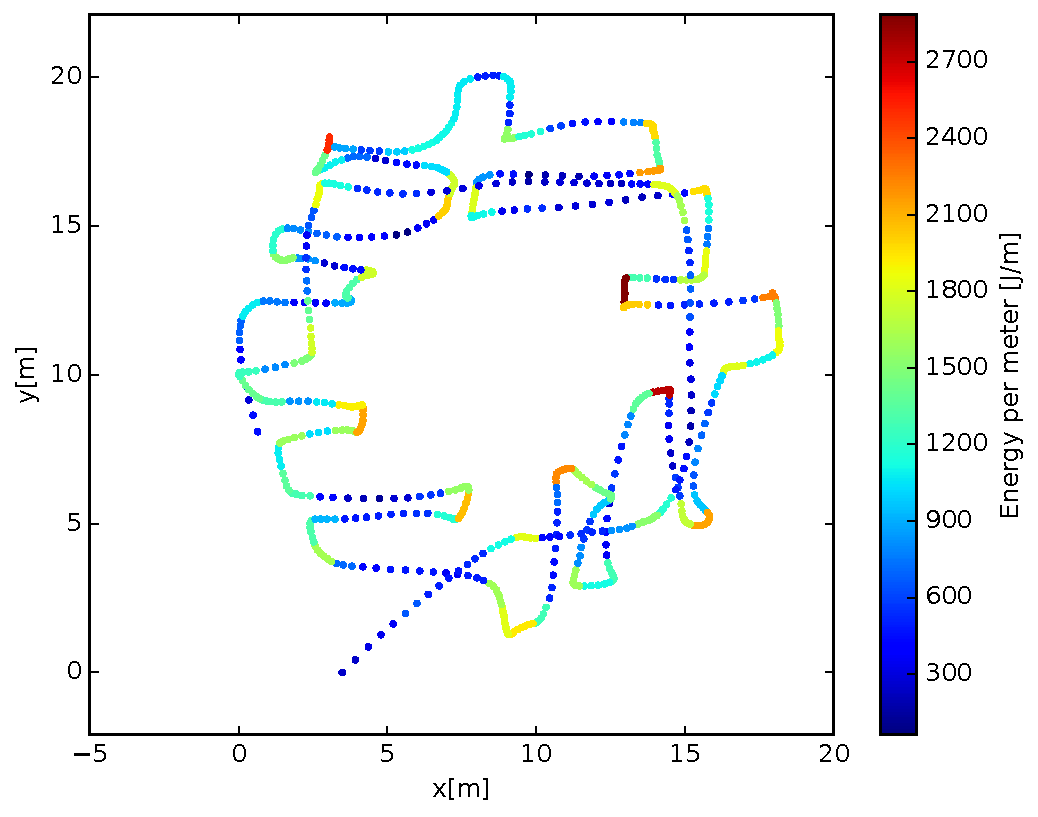
\includegraphics[width=.48\columnwidth]{icra2018/energy_path_2-notype3}
	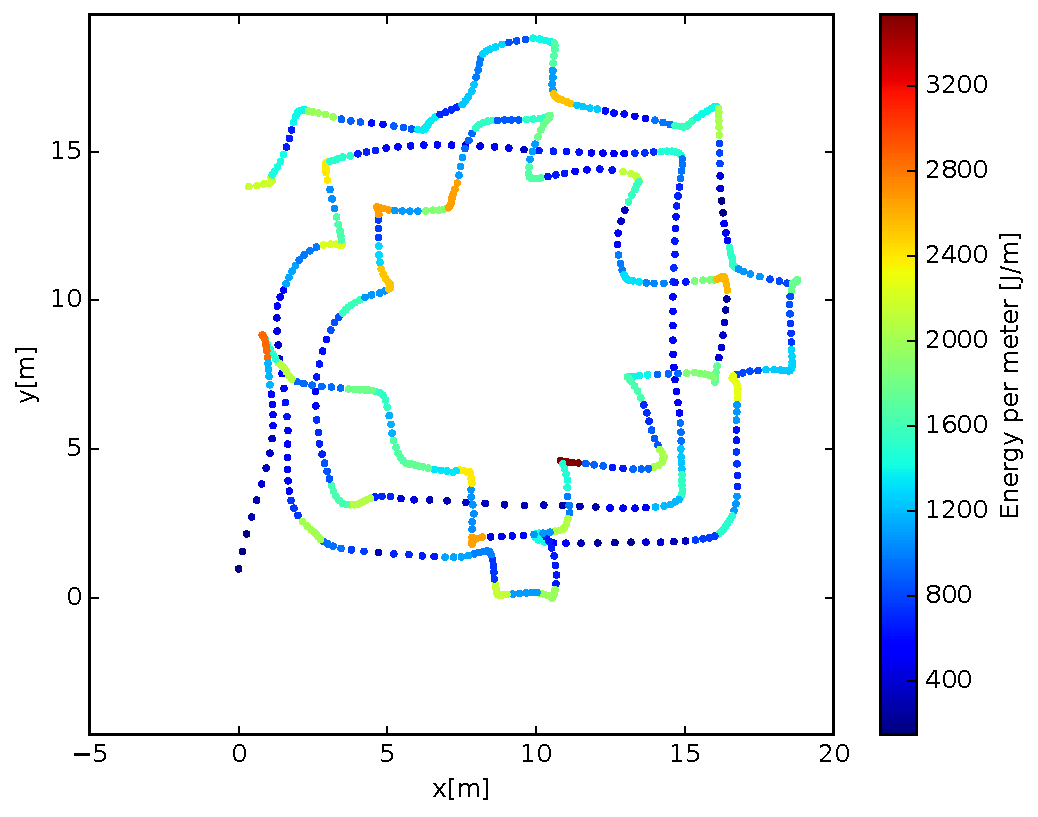
\includegraphics[width=.48\columnwidth]{icra2018/energy_path_3-notype3}
	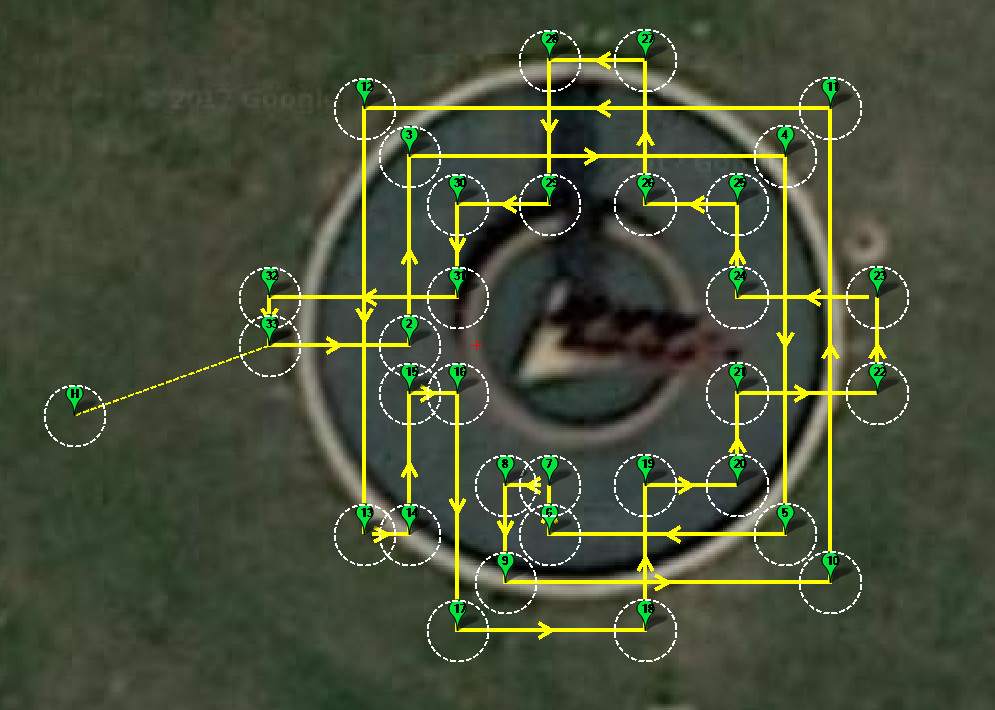
\includegraphics[width=.48\columnwidth]{icra2018/turncost_180}
	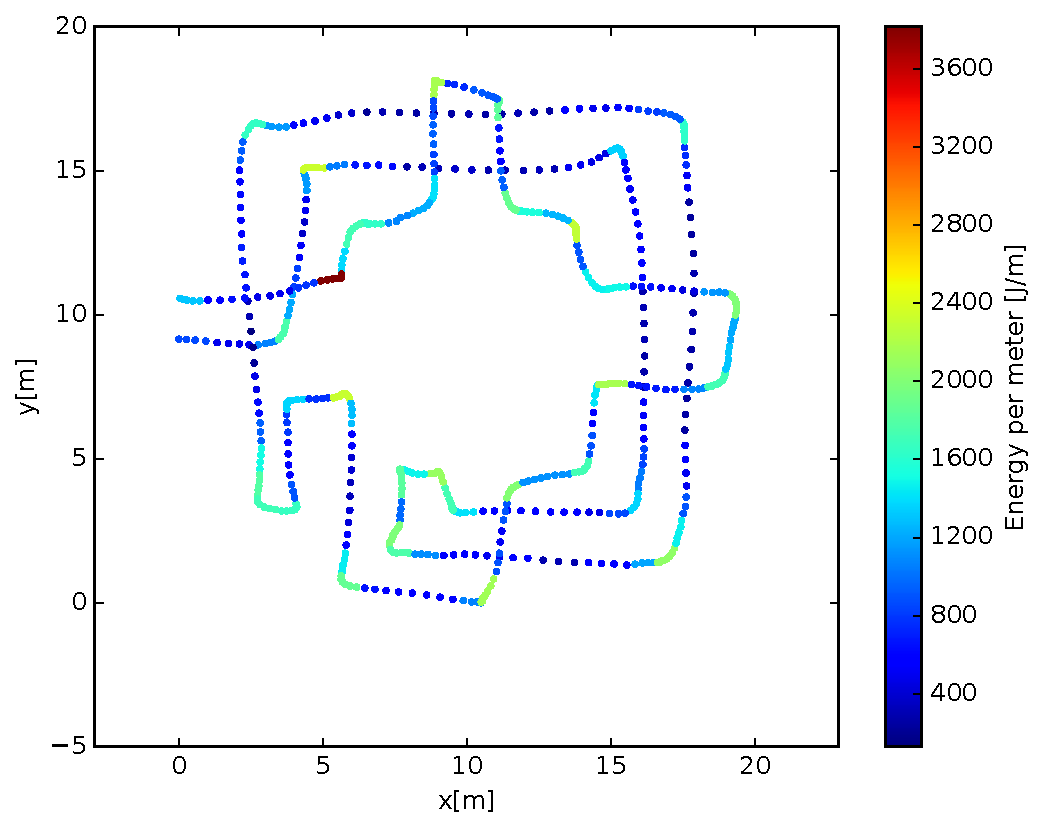
\includegraphics[width=.48\columnwidth]{icra2018/energy_path_1}
	\caption[Fountain]{Paths for an environment surrounding a fountain, which poses an obstacle for the UAV. 
	(Top left) The energy consumption during a real world flight for a boustrophedon path.
	(Top right) The energy consumption during a real world flight for a hand-designed loop path.
	(Bottom left) The optimal penalty cycle cover path.
	(Bottom right) The energy consumption during a real-world flight along the optimal path.} \label{fig:fountain}
	\end{center}
	\vspace{-1em}
\end{figure}


A boustrophedon (back-and-forth) path with \SI{2}{\metre} spacing was generated to cover a region $\SI{120}{\metre} \times \SI{15}{\metre}$ at height $\SI{1.5}{\metre}$.
The path was generated using Mission Planner software from ardupilot.org~\cite{Ardupilot}.

For each trial the UAV took off from a resting position on top of the screen.
Flight began manually, with a piloted takeoff of the UAV. After establishing a stable hover at $\SI{3}{\metre}$, control was switched to the autonomous flight plan.
The pilot monitored the flight with the ability to switch to manual operation in case of potential crashes due to GPS error or hazards in the flight plan.
Mosquito strikes detected by the data logger were verified using a GoPro Hero 4 Silver camera attached at the top of the net, as shown in Fig.~\ref{fig:DroneAndNet}.
At night and twilight, the sparks could be detected both visually and audibly from the recorded video.
During the day, the sparks were loud enough to observe over the audio channel of the videos.

The UAV flew eight missions on this field, covering the same path.
It was mainly flown in the early morning and late afternoon, when mosquito activities are more active.
Three flights were flown at noon and early afternoon to ensure that mosquito activities during these periods were not ignored.
However, only two mosquito strikes were observed during this period.
The path covered is about $\SI{1}{\kilo\metre}$ long and typically takes $\SI{12}{\minute}$.

Over the eight missions on this field, there were a total of 11 mosquito strikes.
Figure \ref{fig:strikemap} shows the mission's flight path and the map of all collected strikes.
The mosquito strikes are concentrated at the north and south ends of the field, where there are more trees.
A density map was generated from the collected strikes' position by representing each strike by a Gaussian distribution with the norm on the strike's location and a $\sigma$ of $\SI{10}{\metre}$.
Figure \ref{fig:densitymap} shows the density map generated by summing these Gaussian distributions.

\begin{figure}
	\centering
	\begin{overpic}[width=1.0\columnwidth]{icra2018/strikeMap.png}\end{overpic}
	\caption{\label{fig:strikemap}
	The UAV's path for flight 3 is in red. Strikes collected along this path are represented by yellow dots.} 
\end{figure}


\begin{figure}
	\centering
	\begin{overpic}[width=1.0\columnwidth]{icra2018/densityMap.pdf}\end{overpic}
	\caption{\label{fig:densitymap} Density map showing mosquito distribution on the field, overlaid by flight path 4 in white. 
	} \vspace{-2em}
\end{figure}

These results not only tell where mosquitoes were but also show where mosquitoes were not.
This is a key difference from stationary traps such as~\cite{chen2014flying,linn2016building}.
Figure~\ref{fig:DroneAndNetOutside} shows the UAV during a dawn flight test near the ocean.    

\begin{figure}
	\centering
	\begin{overpic}[width=1.0\columnwidth]{icra2018/OutdoorMosquitoDrone.jpg}\end{overpic}
	\caption{\label{fig:DroneAndNetOutside}
	The UAV and screen during a flight trial near the ocean.
	} 
\end{figure}

